\documentclass[lmodern, utf8, seminar, numeric]{fer}
\usepackage{booktabs}

\begin{document}

\title{Raspoznavanje preklapajućih 2D objekata}

\author{Tomislav Babić \and Mateja Čuljak \and Đorđe Grbić \and Ivan Krišto \and Maja Šverko}

\maketitle

\tableofcontents


\chapter{Projektni zadatak}

\section{Opis projektnog zadatka}

Cilj projekta je razvijanje sustava računalnog vida za klasifikaciju
preklapajućih $2D$ objekata. Skup objekata koji se klasificiraju je unaprijed
poznat. Pod pojmom ``preklapanje'' uzimaju se u obzir sljedeća pravila:

\begin{itemize}
\item objekti se međusobno preklapaju,
\item moguće je da objekt ne sudjeluje u preklapanju (tj.\ objekt je samostalan),
\item svaki objekt prekriven je najviše jednim objektom,
\item razine preklapanja su proizvoljne,
\item rotacija, skaliranje i pomak objekata su proizvoljni,
\item boja objekta je proizvoljna.
\end{itemize}
Ulaz sustava u fazi inicijalizacije je skup samostalnih objekata koje želimo
klasificirati. U fazi raspoznavanja sustavu predajemo sliku koja sadrži
preklapajuće objekte. Izlaz sustava su nazivi objekata koji se nalaze na slici
te njihove vjerojatnosti da sudjeluju u preklapanju.


\section{Konceptualno rješenje zadatka}

Algoritmi i koncepti korišteni u rješavanju zadatka:
\begin{description}
\item[Binarizacija slike pragom:] Ulazni podatci su slike u \emph{jpg} formatu. Izlazni podatci su binarne slike.
\item[Izlučivanje značajki:]  Riječ je zapravo o pronalasku linearnih segmenata konture u sceni, odnosno pronalasku rubova u sceni te aproksimacija rubova poligonima. Ulazni podatci su binarne slike, a izlaz vektor segmenata.
\item[Generiranje hipoteza:] Usporedba linearnih segmenata konture u slici sa segmentima iz modela u bazi podataka skupa za učenje. Ulazni podatci su vektori segmenata, a izlazni podatci generirane hipoteze, točnije, mjere sličnosti kompatibilnih linearnih segmenata.
\item[Evaluacija hipoteza:] Nakon generiranja hipoteza potrebno je iste evaluirati. Odnosno, usporediti i ostale linearne segmente sa segmentima modela. Ulazne podatke predstavljaju generirane hipoteze, a izlazni podatci su hipoteze sortirane na način da prva odgovara najbolje procijenjenoj hipotezi, a posljednja najgore procijenjenoj hipotezi.
\end{description}

Izlaz sustava su nazivi klasa objekata (iz najbolje procijenjenih hipoteza) koji
sudjeluju u preklapanju unutar nove scene.


\chapter{Postupak rješavanja zadatka}

Sustav je zamišljen tako da se sastoji od četiri osnovne komponente:
\begin{itemize}
\item komponente za učitavanje i spremanje slika,
\item filtera slika,
\item vaditelja značajki objekata na slikama,
\item algoritma za raspoznavanje.
\end{itemize}

Filter slika priprema slike za postupak vađenja značajki, primjerice, pretvara
RGB sliku u binarnu. Vaditelj značajki zapisuje objekte na slikama u format
prilagođen algoritmu raspoznavanja.

Sustav raspoznavanja treba biti robustan i otporan na što veći broj
konfiguracija preklapanja. Navedeni zahtjev podrazumijeva da će algoritam
raspoznavanja te značajke koje on koristi moći nesmetano funkcionarati i u
uvjetima kad su:

\begin{itemize}
\item objekti proizvoljno rotirani,
\item objekti proizvoljno skalirani,
\item objekti proizvoljno smješteni u ravnini,
\item površine preklapanja različite,
\item objekti jednake boje.
\end{itemize}

Opisan rad sustava možemo promatrati kroz dva koraka -- inicijalizaciju i
raspoznavanje objekata scene. Prilikom inicijalizacije, za svaki objekt koji
želimo klasificirati sustavu predočavamo scenu koja sadrži samo taj objekt.
Sustav vadi značajke i sprema ih. U koraku raspoznavanja, sustav na ulazu dobiva
sliku scene u kojoj se nalaze preklopljeni objekti, koristi spremljene značajke
nepreklopljenih objekata, vadi značajke objekata unutar nove scene te uspoređuje
značajke objekata nove scene sa spremljenim značajkama. Navedeni korak rješenja
se zasniva na konceptima opisanim u \citep{ayache2009hyper}.


\section{Poligonizacija objekata}

\subsection{Dobivanje binarne slike iz slike u boji}
Slika u boji se prvo pretvara u sivu sliku, gdje se vrijednost slikovnog
elementa sive slike računa kao vrijednost osvijetljenosti \engl{luminance} 
$s$ na sljedeći način:
$$s = r \cdot 0.3 + g \cdot 0.59 + b \cdot 0.1,$$
gdje su $r$, $g$ i $b$ komponente slikovnog elementa slike u RGB prostoru boja.
Nakon toga se siva slika pretvara u binarnu. Slikovni element se uspoređuje s
pragom te ako mu je vrijednost veća od praga, tada će on poprimiti iznos jednak
nuli. U suprotnom slučaju slikovni element poprima vrijednost 255.

\subsection{Algoritam za praćenje granice}
Algoritam se izvodi na sljedeći način:
\begin{enumerate}
  \item Provjeriti sastoji li se objekt od jednog izoliranog slikovnog elementa. Ako je to istina, taj element je ujedno i granica. U tom slučaju zaustaviti postupak.
  \item Pretraživanjem slike naći dva susjedna elementa, $c \in S$ i $d \in \bar S$, pri čemu je $S$ skup točaka koje pripadaju objektu (povezanoj slikovnoj komponenti).
  \item Promijeniti vrijednost točke $c$ u 3, a točke $d$ u 2.
  \item Označiti 8-susjedstvo točke $c$ sa $e_1, e_2, \ldots ,e_k$ počevši od točke $d$, u smjeru kazaljke na satu, i zaustavivši se s prvim pojavljivanjem broja 1, 3 ili 4.
  \item Ako je $c=3, e_k=4, e_h=2$ za neki $h<k$, promijeni 3 u 4, 2 u 0 te se zaustavi.
  \item Inače, promijeni vrijednost $c$ u 4, ako je prije toga imao vrijednost 1. Kao novu vrijednost za $c$ uzmi $e_k$, a za $d$ uzmi $e_{k-1}$. Ponavljaj sve od 4.\ koraka.
\end{enumerate}
Nakon završetka algoritma, slikovni elementi koji imaju vrijednost 4 predstavljaju granicu objekta.

\subsection{Podijeli i vladaj algoritam za segmentaciju ruba}
Algoritam podijeli-i-vladaj se koristi kad se rub može prikazati jednostavnijim funkcijskim oblicima, te kad su poznate krajnje točke granice (dva rubna elementa).

Algoritam se izvodi na sljedeći način:
\begin{enumerate}
  \item
Povući pravocrtnu liniju između dvije krajnje točke granice.
   \item Izračunati pravokutne udaljenosti za svaki slikovni element koji je rubni element i nalazi se u području granice.
   \item Usporediti dobivene udaljenosti s unaprijed zadanim pragom $\tau$.
   \item Ako su sve udaljenosti manje od $\tau$, zaustaviti algoritam.
   \item Rubni element s najvećom udaljenošću postaje prijelomna točka. Prošli linijski segment se zamjenjuje s novim linijskim segmentima (tj.\ linijama od krajnjih točaka prema prijelomnoj točki).
   \item Rekurzivno izvesti algoritam koristeći nove linijske segmente.
\end{enumerate}

Eksperimentalno je odabran prag $\tau$ u iznosu od 10 piksela.

Točke pronađene algoritmom praćenja granica se dijele na dva skupa. Prvi skup
obuhvaća sve točke od prve do središnje, a drugi skup obuhvaća preostali skup
točaka. Podijeli i vladaj algoritam se izvodi nad oba skupa zasebno te se
dobivaju dva skupa linearnih segmenata. Kako bi se dva skupa spojila u jedan,
potrebno je spojiti uzastopne segmente slične orijentacije. Ako je razlika
orijentacija manja od zadanog praga, segmenti se spajaju. Prag korišten u
implementaciji postupka iznosi 15 stupnjeva.


\section{Generiranje hipoteza}
Ulazni skup podataka prilikom generiranja hipoteza čine vektori segmenata slika
za učenje (u daljem tekstu slike modela) i slika za testiranje (u daljnjem
tekstu slike scene). Svaka hipoteza je zapravo pretpostavka da određen segment
scene odgovara određenom segmentu modela. U obzir se pritom uzimaju samo
kompatibilni segmenti. Kompatibilnost je u ovom slučaju definirana dvama
pragovima. Prvi prag određuje razliku među kutovima $A$ između segmenta modela i
njegovog prethodnika te kuta $A'$ između segmenta scene i njegovog prethodnika.
Drugi prag određuje omjer u duljini dvaju segmenata.


Transformacija $T$ koja može poslužiti za olakšavanje usporedbe dvaju segmenata
definirana je u literaturi \citep{ayache2009hyper} i glasi ovako:

\begin{align}
x^{\ast} & = tx + x\cdot k\cdot \cos(\beta) - y\cdot k\cdot \sin(\beta), \\
y^{\ast} & = ty + y\cdot k\cdot \cos(\beta) + y\cdot k\cdot \sin(\beta).
\end{align}

Koeficijenti $tx$, $ty$, $k$ i $\beta$ mogu se izračunati na sljedeći način:
\begin{align}
k & = l(S_i)/l(M_i),\\
\beta & = a(S_i) - a(M_i),\\
tx & = x' - k\cdot ( x \cdot \cos(\beta) - y\cdot \sin(\beta)), \\
ty & = y' - k\cdot ( x \cdot \sin(\beta) + y\cdot \cos(\beta)),
\end{align}
gdje je $S_i$ linearni segment u sceni, $M_i$ linearni segment modela, $l$ je
duljina segmenta, $\beta$ je kut između segmenta i horizontalne osi, a $x'$, $y'$
predstavljaju koordinate središnjih točaka segmenta.
Generirane hipoteze spremaju se u vektor hipoteza.

\section{Evaluacija hipoteza}
\subsection{Sparivanje dodatnih linearnih segmenata}
Nakon generiranja hipoteza potrebno je iste evaluirati, pri čemu se iterativno uspoređuju preostali linearni segmenti modela sa segmentima scene.

\begin{figure}[htb]
\begin{center}
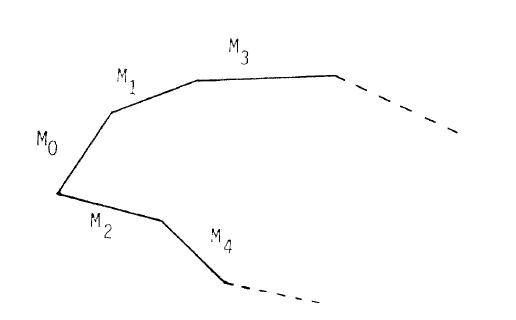
\includegraphics[width=6cm]{resources/segmenti.png}
\end{center}
\caption{Redoslijed odabira segmenata iz modela.}
\label{fig:redoslijed_odabira}
\end{figure}

Algoritam u svakoj iteraciji odabire segment $M_i$ iz modela (slika
\ref{fig:redoslijed_odabira}) i izračunava njegov položaj u sceni trenutnom
transformacijom. Nakon toga se uspoređuje različitost transformiranog segmenta
modela, $tM_i$ sa svakim segmentom u sceni, $S_j$. Mjera sličnosti $d_{ij}$
između segmenata $tM_i$ i $S_j$ može se izraziti pomoću tri mjere:

\begin{enumerate}
  \item $a_{ij}$ je mjera koja se računa kao apsolutna vrijednost razlike između segmenata $tM_i$ i $S_j$,
  \item $D_{ij}$
se računa kao Euklidska udaljenost između središnjih točaka segmenata $tM_i$ i $S_j$,
  \item $l_{ij}$ se računa kao relativna udaljenost između duljina segmenata $tM_i$ i $S_j$ te odgovara sljedećem izrazu: $l_{ij}=(l_i'-l_j)/l_j$, gdje je $l_i'$ duljina segmenta $tM_i$, a $l_j$ duljina segmenta $S_j$.
\end{enumerate}

Svaka od tih mjera ograničena je pripadnom gornjom vrijednošću $a_{Max}$,
$D_{Max}$ ili $l_{Max}$ koje u trenutnoj implementaciji iznose: $a_{Max}=0.35$,
$D_{Max}=45$ ili $l_{Max}=0.7$.


Ukoliko neka od tih mjera ima iznos veći od svoje gornje granice, tada je
$d_{ij}=1$, inače mjera različitosti se računa na sljedeći način:
\begin{equation}
d_{ij}=p\cdot a_{ij}/a_{Max}+q\cdot D_{ij}/D_{Max}+r\cdot l_{ij}/l_{Max},
\end{equation}
gdje su $p,q,r$ pozitivne težine čija suma iznosi 1. U trenutnoj implementaciji
njihove vrijednosti su: $p=0.6$, $q =0.3$, $r=0.1$.

Segment $M_i$ je sparen sa segmentom $S_j$ kada je $d_{ij}$ najmanjeg iznosa i
manji od 1. Ukoliko za nijedan segment scene $S_j$, $d_{ij}$ nije iznosa manjeg
od 1, tada segment $M_i$ nema par u sceni.


\subsection{Ažuriranje transformacije}
Nakon što su segmenti $M_i$ i $S_j$ spareni, potrebno je izvršiti ažuriranje
hipoteze korištenjem rekurzivne metode najmanjih kvadrata. Cilj je pronaći
transfomaciju $T$ koja minimizira kriterij:
$$R=\sum_i \frac{l_i}{K}\Delta^2(T(m_i),s_{ji}),$$
gdje su $m_i$ i $s_{ji}$ središnje točke segmenata $M_i$ i $S_j$. $\Delta$ je
oznaka za euklidsku udaljenost, dok je $l_i$ duljina segmenta $M_i$. $K$ je
konstanta koja se u trenutnoj implementaciji dobiva izrazom: $K = D_{Max}\cdot
l_{Mean}$, gdje je $l_{Mean}$ prosječna duljina segmenata u modelu, a $D_{Max}$
je definiran u prethodnom potpoglavlju.


Ako predstavimo transformaciju $T$ pomoću vektora
$$ v=(k\cdot  \cos\beta, k\cdot \sin\beta, tx,t y)^T$$
te točku $s_{ji}$  s koordinatama $x_i'$ i $y_i'$
predstavimo vektorom ${Y_i}=(x_i',y_i')^T$ možemo prethodni izraz zapisati
kao:
$$R=\sum_i({Y_i}-C_i v)^T W_i^{-1}({Y_i}-C_i v).$$
Matrica $C_i$ je dana sljedećim izrazom:
$$C_i = \left [ \begin{array}{cccc}
x_i & -y_i & 1 & 0\\
y_i & x_i & 0 & 1
\end{array} \right ],$$
gdje su $x_i$ i $y_i$ koordinate središnje točke segmenta modela $m_i$. Matrica $W_i$ je dana izrazom:
$$W_i = \left [ \begin{array}{cc}
w_i^2 & 0\\
0 & w_i^2
\end{array} \right ],$$
gdje vrijedi $w_i = K/l_i$.

Kako bi se mogli kontrolirati parametri transformacije $T$, u minimizacijski kriterij dodan je dodatni član, pa se izraz naposlijetku može zapisati na sljedeći način:
$$R=\sum_i({Y_i}-C_i v)^T W_i^{-1}({Y_i}-C_i v)+( v -  v_0)^T S_0^{-1}( v- v_0).$$
$R$ je kvadratni kriterij koji se može rekurzivno minimizirati sljedećim jednadžbama:
\begin{align*}
v_i & = v_{i-1}+K_i(Y_i-C_i\cdot v_i),\\
K_i & = S_{i-1}C_i^T(W_i+C_iS_{i-1}C_i^T)^{-1},\\
S_i & = (l+K_iC_i)S_{i-1}.
\end{align*}
Ove jednadžbe se inicijaliziraju za svaku hipotezu te se rekurzivno ažuriraju nakon svakog sparivanja segmenata modela i scene.

\chapter{Evaluacija rješenja}
\section{Opis baze uzoraka}
Baza uzoraka sastoji se od 120 slika koje sadrže dvanaest različitih oblika
izrađenih od tvrdog papira; šest jednostavnijih i šest kompleksnijih. Za svaki
od dvanaest oblika postoji 10 slika; dvije slike samog oblika (različite po
veličini, rotaciji i translaciji) i 8 različitih slika oblika prekrivenog drugim
oblikom. Dimenzije uzoraka su $900 \times 600$ piksela. Oblici se jasno
razaznaju od pozadine, no ponegdje bacaju blijedu sjenu zbog blage savijenosti
oblika. Sve slike preklapanja sadrže oblike različitih boja, međutim u
implementaciji rada se ta informacija ne koristi.

Imenovanje scene je vršeno po formatu ``\texttt{m1m2[a-z].jpg}''. Oznaka
\texttt{m1} označava kod donjeg modela (npr.\ 12 za kapljicu, 01 za kvadrat),
\texttt{m2} gornjeg modela, ``\texttt{[a-z]}'' broj pojave kombinacije --
primjerice ako se pojavljuju dvije scene u kojima je kapljica na kvadratu, tada
imamo scene \texttt{0112a.jpg} i \texttt{0112b.jpg}. Nepravilnost u formatu
postoji kod oznake modela i njegovog transformiranog oblika. Oznaka
\texttt{m100} označava samostalni transformirani (rotirani, skalirani i malo
translatiran) objekt, a oznaka \texttt{m101} \textbf{ne označava} kvadrat na modelu
\texttt{m1} već sam model. Kvadrat na modelu \texttt{m1} označava se dodatnim
slovima, odnosno: \texttt{m101.jpg} je slika modela, ali \texttt{m101a.jpg} je
slika kvadrata na modelu.

\begin{figure}[htb]
\begin{center}
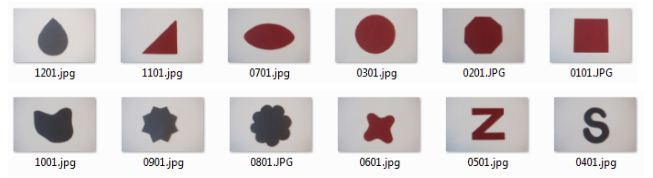
\includegraphics[width=13.5cm]{resources/baza.png}
\end{center}
\caption{Prikaz objekata za klasifikaciju.} 
\label{fig:baza}
\end{figure}

\section{Rezultati i analiza evaluacije}
Pri evaluaciji korištene su sve slike iz baze izuzev slika na kojima se
pojavljuje trokut zbog prevelike sličnosti s pravokutnikom. Za svaku scenu
(sliku preklapanja objekata) provedena je evaluacija u kojoj je sudjelovalo 11
modela (svi osim trokuta). Rezultat evaluacije su vjerojatnosti da se određeni
model nalazi na sceni.

Problemi rotacije, skaliranja i translacije objekata javljaju se u samom početku
obrade scene. Navedeni problemi su rješivi odabirom značajki koje su
invarijantne na njih te dobrim parametrima metoda koje se koriste za izgradnju
značajki (primjerice, poligonizaciju slike). Pri evaluaciji, parametri nisu
varirani već su eksperimentalno odabrani parametri koji su se pokazali relativno
dobrima (navedeni su uz svaku metodu u ostatku dokumentacije).

Bitno je napomenuti da je metoda izuzetno ovisna o prirodi baze modela i scena
na koje je primjenjena, odnosno sličnostima među modelima u bazi te načinu
preklapanja objekata u sceni. Složenost modela može poboljšati uspješnost
klasifikacije jer se klasifikacija temelji na uspoređivanju sličnosti objekata i
modela.

Mjera kvalitete pojedine hipoteze je izražena omjerom duljine segmenata modela
sparenih s odgovarajućim segmentima u sceni te duljine svih segmenata modela.
Maksimalna vrijednost kvalitete hipoteze je 1 te se ona postiže samo kada su svi
segmenti modela spareni sa odgovarajućim segmentima scene.

Prikaz uspješnosti prepoznavanja pojedinog modela unutar scene može se vidjeti
po brojevima uspješnih i neuspješnih prepoznavanja na slici \ref{fig:graf}.

\begin{figure}[htb]
\begin{center}
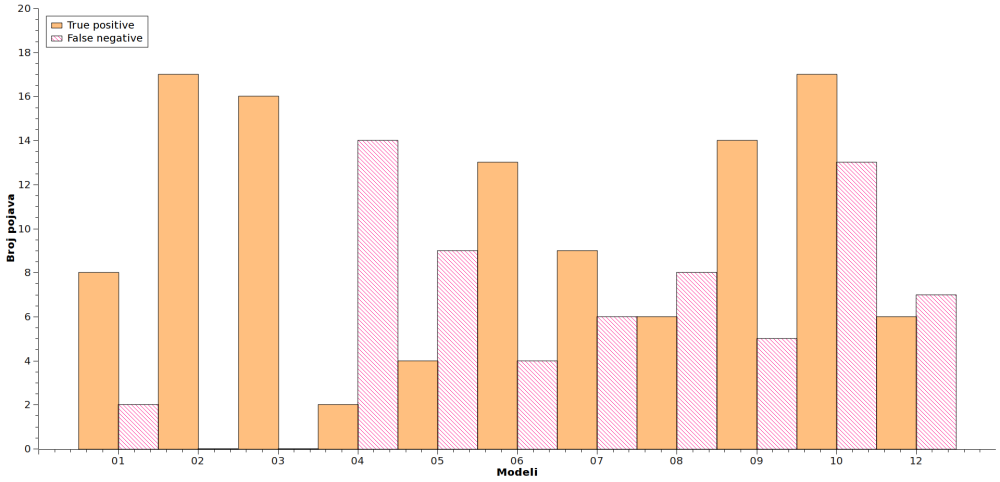
\includegraphics[width=15cm]{resources/graf.png}
\end{center}
\caption{Graf uspješnih i neuspješnih prepoznavanja po modelima.} 
\label{fig:graf}
\end{figure}

Statistika je prikazana tablicama \ref{tbl:po-hipot} i \ref{tbl:po-obj}. Tablica
\ref{tbl:po-hipot} prikazuje uspješnost prepoznavanja povezanu sa brojem
najbolje rangiranih (najvjerojatnijih) hipoteza. Kod tablice \ref{tbl:po-obj},
uzeta je pretpostavka da svaka scena sadrži jedan objekt ili dva različita te je
prikazana statistika uspješnosti prepoznavanja po broju prepoznatih objekata (s
lijeve strane je broj uspješno prepoznatih objekata, dok je s desne broj
objekata na slici). Iz tablice \ref{tbl:po-obj} možemo zaključiti da se svi
objekti na sceni prepoznaju u $40\%$ slučajeva, neovisno o tome sadrži li scena
1 ili 2 objekta. Barem jedan objekt na sceni se prepozna u $86.7\%$ slučajeva
(radi se o stupcima ``1 od 1'', ``1 od 2'' i ``2 od 2'' u tablici
\ref{tbl:po-obj}).
Tablica \ref{tbl:po-hipot} je napravljena koristeći 83 slike, tablica
\ref{tbl:po-obj} koristeći 105 slika. Pri izgradnji tablice \ref{tbl:po-obj} kao
scene korišteni su i sami modeli (nema striktnog učenja te hold-out metoda nije
neophodna). Time je metoda evaluirana za prepoznavanje nepreklopljenog objekta.

\begin{table}[htb]
\centering
\caption{Uspješnost prepoznavanja po hipotezama.}
\label{tbl:po-hipot}
\begin{tabular}{l l l l l}
\toprule
 & 2/2 & 2/3 & 2/4 & 1/2\\
\midrule
Broj: & 22 & 42 & 52 & 77\\
Postotak: & $26.5\%$ & $50.6\%$ & $62.5\%$ & $92.8\%$\\
\bottomrule
\end{tabular}
\end{table}

\textbf{Objašnjenje mjera:}
\begin{itemize}
    \item 2/2 znači da su dva najbolja prijavljena objekta ispravni (dva istinito pozitivna objekta),
    \item 2/3 znači da su među tri najbolja prijavljena objekta dva ispravna (uključuje prijavljene objekte iz prethodne mjere),
    \item 2/4 znači da su među četiri najbolja prijavljena objekta sigurno dva ispravna (uključuje prijavljene objekte iz obje prethodne mjere),
    \item 1/2 znači da je među dva najbolja prijavljena objekta sigurno jedan ispravan (uključuje prijavljene objekte iz svih prethodnih mjera).
\end{itemize}

\begin{table}[htb]
\centering
\caption{Uspješnost prepoznavanja po objektima.}
\label{tbl:po-obj}
\begin{tabular}{l l l l l l}
\toprule
 & 1 od 1 & 0 od 1 & 2 od 2 & 1 od 2 & 0 od 2\\
\midrule
Broj: & 21/22 & 1/28 & 21/83 & 49/83 & 7/83\\
Postotak: & $95.4\%$ & $3.6\%$ & $25.3\%$ & $59.0\%$ & $8.4\%$\\
\bottomrule
\end{tabular}
\end{table}

U nastavku je dan pokazni primjer za jednu scenu. Na sceni se preklapaju objekt
s konturom elipse i zvijezda s osam vrhova, kao što se može vidjeti na slici \ref{fig:scena-preklapanja}.

\begin{figure}[!h]
\begin{center}
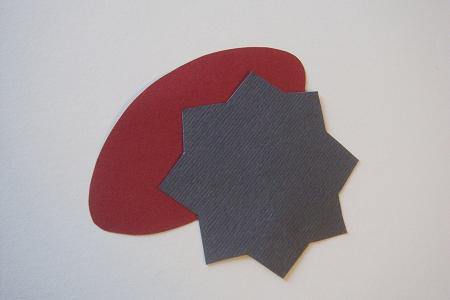
\includegraphics[width=9cm]{resources/spoj.png}
\end{center}
\caption{Scena s dva preklapajuća objekta koji odgovaraju modelima 0701 i 0901.} 
\label{fig:scena-preklapanja}
\end{figure}

\begin{figure}[!h]
\begin{center}
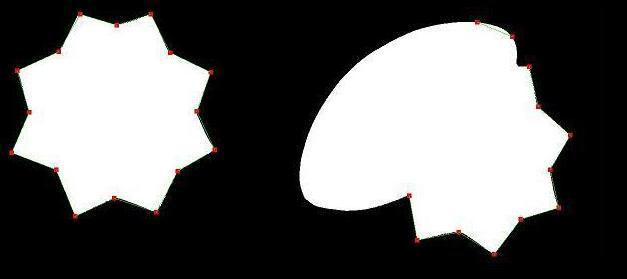
\includegraphics[width=11cm]{resources/zvijezda-spoj.png}
\end{center}
\caption{Prikazani segmenti na modelu (lijevo) i sceni (desno) za najbolju hipotezu.} 
\label{fig:segmenti-na-modelu}
\end{figure}

Prva hipoteza tvrdi da se na sceni nalazi zvijezda s kvalitetom iznosa $63.9\%$.
Možemo vidjeti kako su svi vidljivi segmenti zvijezde u sceni ispravno
pronađeni, te da je pogrešno detektiran još jedan segment na rubu elipse. Razlog
tome je u iznosu parametra $D_{Max}$ koji određuje maksimalnu dopuštenu udaljenost
između transformiranog segmenta modela i segmenta scene. S povećanjem tog
parametra, rasti će i broj pogrešno detektiranih segmenata. Smanjenjem tog
parametra se smanjuje broj ispravno detektiranih segmenata.

\begin{figure}[!h]
\begin{center}
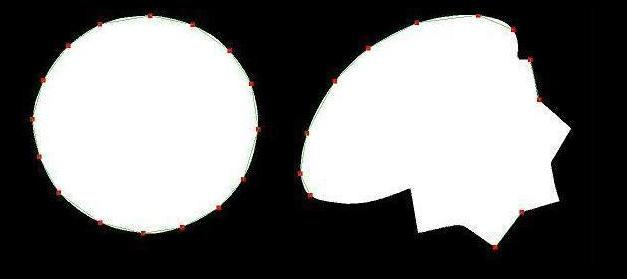
\includegraphics[width=11cm]{resources/krug-spoj.png}
\end{center}
\caption{Prikazani segmenti na modelu (lijevo) i sceni (desno) za drugu najbolju hipotezu.} 
\label{fig:segmenti-druga-naj}
\end{figure}

Druga hipoteza tvrdi da se na sceni nalazi krug s kvalitetom iznosa $54.8\%$. Na
sceni se krug ne nalazi, ali valja primijetiti kako kontura elipse odgovara
dijelu luka kod kružnice. Možemo vidjeti da postupak detektira još dva segmenta
(na području zvijezde) koji bi mogli pripadati toj zamišljenoj kružnici.

\begin{figure}[!h]
\begin{center}
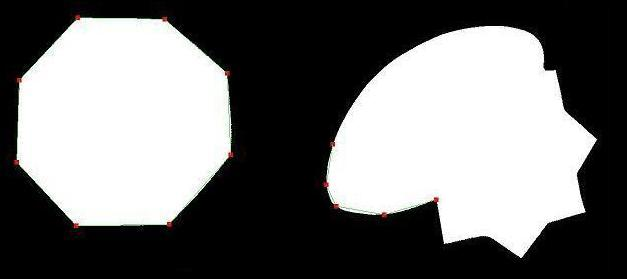
\includegraphics[width=11cm]{resources/oktagon-spoj.png}
\end{center}
\caption{Prikazani segmenti na modelu (lijevo) i sceni (desno) za treću najbolju hipotezu.} 
\label{fig:segmenti-treca}
\end{figure}

Treća hipoteza tvrdi da se na sceni nalazi osmerokut s kvalitetom iznosa $50.3\%$.
Kao i u prethodnom slučaju, osmerokut nije na sceni. Razlog pogrešci je sličan
kao i u prethodnom slučaju tj.\ segmenti osmerokuta odgovaraju, unutar dozvoljene
pogreške, dijelu elipse nakon rubne segmentacije.

\begin{figure}[!h]
\begin{center}
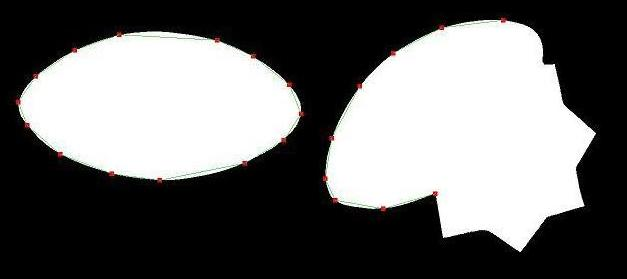
\includegraphics[width=11cm]{resources/elipsa-spoj.png}
\end{center}
\caption{Prikazani segmenti na modelu (lijevo) i sceni (desno) za četvrtu najbolju hipotezu.} 
\label{fig:segmenti-cetvrta}
\end{figure}

Četvrta hipoteza tvrdi da se na sceni nalazi elipsa s kvalitetom iznosa $49.5\%$.
To je ispravna hipoteza, te možemo vidjeti kako je velik broj segmenata u sceni
ispravno detektiran, ali je i određen dio promašen. Do pogreške je došlo zbog
postupka rubne segmentacije. Može se primijetiti kako su na modelu elipse dva
segmenta duža i udaljenija od konture elipse, nego što je to slučaj s ostalim
segmentima. Razlog tome je što implementacija postupka rubne segmentacije
(podijeli i vladaj) u ovom radu nije u potpunosti invarijantna na skaliranje i
rotaciju. S obzirom na malu razliku u vjerojatnostima između druge, treće i
četvrte hipoteze, ispravna detekcija preostalih segmenata, mogla je dovesti do
toga da prve dvije hipoteze budu ispravne.

Spajanje segmenata je nužno zbog toga što nije pronađen način za pronalazak
idealnih početnih rubnih točaka u postupku segmentacije. Posljedica je prevelik
broj linearnih segmenata od stvarnog broja, što dovodi do pogreške u postupku
evaluacije hipoteza. Međutim, ukoliko je kriterij prilikom usporedbe previše
blag, tada će se segmenti koji nemaju sličnu orijentaciju spojiti te će se
dogoditi pogreška u postupku evaluacije hipoteza. U trenutnoj implementaciji
kriterij je utvrđen kao razlika između orijentacija susjednih segmenata. Ukoliko
je razlika manja od praga, koji iznosi 15 stupnjeva, tada se segmenti spajaju.

Primjer kako rotacija utječe na postupak rubne segmentacije može se vidjeti na
slici \ref{fig:segmenti-rotacija}.

\begin{figure}[!h]
\begin{center}
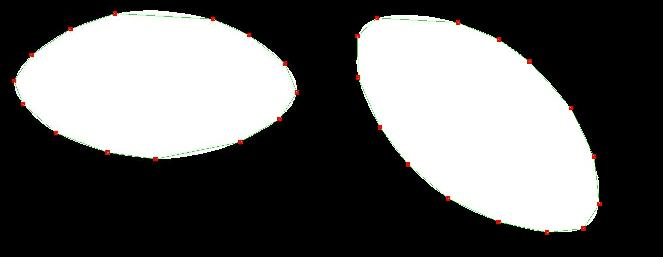
\includegraphics[width=11cm]{resources/dvije-elipse.png}
\end{center}
\caption{Lijevo je prikazan model elipse (0701), a desno je prikazan isti model nakon rotacije.} 
\label{fig:segmenti-rotacija}
\end{figure}

\chapter{Opis programske implementacije}
Implementacija je izvedena u programskom jeziku C++ koristeći Microsoft Visual
Studio razvojno okruženje. Sustav razložen po komponentama može se vidjeti na
slici \ref{fig:komponente}.

\begin{figure}[htb]
\begin{center}
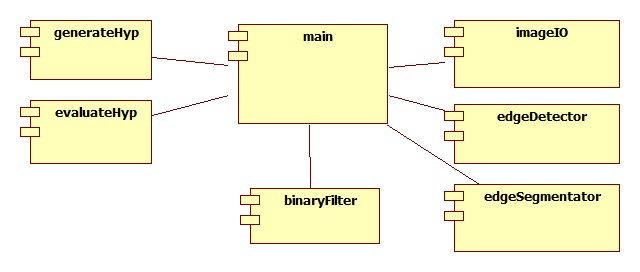
\includegraphics[width=11cm]{resources/komponente.png}
\end{center}
\caption{Sustav razložen po komponentama.} 
\label{fig:komponente}
\end{figure}

Za učitavanje slika koristi se OpenCV biblioteka\footnote{\url{http://opencv.willowgarage.com/wiki/}}, dok se za operacije s
matricama koriste biblioteke Boost, Template Numerical Toolkit (TNT) i JAMA/C++
Linear Algebra Package koje su dostupne na:
\begin{itemize}
  \item \url{http://www.boost.org/},
  \item \url{http://math.nist.gov/tnt/download.html} (TNT i jama).
\end{itemize}
Trenutno je moguće učitati slike isključivo u \emph{jpg} formatu. Jedno od
potencijalnih poboljšanja sustava jest uklanjanje ovisnosti o OpenCV biblioteci
te povećanje broja formata koje sustav može koristiti (npr.\ uvođenje \emph{libpng},
\emph{libjpg} i sličnih biblioteka umjesto glomazne OpenCV biblioteke).

\section{Pokretanje implementacije}
Implementacija se pokreće iz komandne linije, primjerice:
\begin{verbatim}
overlaping_obj_det.exe --modelsdir ../baza/ --scenepath \
../baza/0102.jpg -m 0101.jpg,1201.jpg
\end{verbatim}
Obavezni parametri su:
\begin{itemize}
  \item putanja do direktorija s bazom (\texttt{modelsdir} ili \texttt{b}),
  \item putanja do slike sa scenom (\texttt{scenepath} ili \texttt{s}),
  \item lista slika modela (\texttt{models} ili \texttt{m}).
\end{itemize}
Popis svih parametara može se dobiti pozivom:
\begin{verbatim}
overlaping_obj_det.exe -h
\end{verbatim}
% Rezultati:
% \begin{verbatim}
% Usage: overlaping_obj_det.exe [options]
% --help,           -h          Displays this message
% --polyangle,      -a <args>   (float) Threshold angle for connecting
% polygons.
% --polydotdist,    -i <args>   (int) Threshold for connecting dots
% into polygons.
% --hypcompangle,   -c <args>   (float) Threshold angle for compatible
% hypotesis.
% --hypcomplength,  -l <args>   (float) Threshold length for compatible
% hypotesis.
% --scenesegsnum,   -g <args>   (int) Number of segments in scene.
% --modelsegsnum,   -j <args>   (int) Number of segments in model.
% --hypsnum,        -f <args>   (int) Number of hypotesis.
% --modelsdir,      -b <args>   [REQUIRED] Path to directory with models
% (must end with '/').
% --scenepath,      -s <args>   [REQUIRED] Path to scene image.
% --models,         -m <args>   [REQUIRED] List of models (filenames).
% Format: name1.jpg,name2.jpg,name3.jpg
% --verbose,        -v          Verbose output.
% \end{verbatim}

Neobavezni parametri imaju svoje predefinirane vrijednosti. No ako se koriste
drugi modeli, variranje parametara može poboljšati uspješnost postupka.
Program ispisuje iznos vjerojatnosti da se pojedini model nalazi na sceni,
primjerice:
\begin{verbatim}
1.)0101.jpg 1
2.)1201.jpg 0.335778
\end{verbatim}
\textbf{NAPOMENA:} Implementacija zahtjeva OpenCV biblioteku na računalu. Ako na računalu
nije instaliran OpenCV i nemate želju instalirati ga, onda kopirajte dll
datoteke: cv210.dll, cv210d.dll, cvaux210.dll, cvaux210d.dll, cxcore210.dll,
cxcore210d.dll, cxts210.dll, highgui210.dll, highgui210d.dll, ml210.dll,
ml210d.dll, opencv\_ffmpeg210.dll, opencv\_ffmpeg210d.dll, u direktorij:\\
\verb|c:\Windows\System32|.

\section{Prevođenje programskog koda}
Programsko rješenje trenutno je prilagođeno samo za Visual Studio prevoditelj,
no moguće ga je prepraviti na način da se omogući i prevođenje preko drugih
prevoditelja (primjerice, g++ prevoditelja).

Prije postupka prevođenja potrebno je instalirati OpenCV 2.1, skinuti Boost 1.4,
TNT i JAMA biblioteke te ih raspakirati na disk. Pazite da direktoriji u koji
instalirate OpenCV i direktoriji u koji raspakirate preostale biblioteke nemaju
prazinu u nazivu (znači, ``Program Files'' direktorij nije dobar izbor). Po
koracima:
\begin{enumerate}
  \item instalirajte OpenCV 2.1 (npr.\ u direktorij \verb|C:\OpenCV2.1|),
  \item raspakirajte Boost (npr. u direktorij \verb|C:\includes|),
  \item raspakirajte TNT i JAMA arhivu (npr. u direktorij
  \verb|C:\includes\tnt|) -- direktorij u koji raspakirate te datoteke \textbf{mora} se
  zvati ``tnt'' i mora sadržavati samo header (.h) datoteke TNT i JAMA
  biblioteka,
  \item stvorite novi Visual Studio C++ \emph{Win32 Console Application} projekt i
  odaberite da se radi o ``empty'' projektu (da VS ne generira nepotreban kod),
  \item u \emph{Source Files} i \emph{Header Files} dodajte postojeći kod (pazite da kod
  unutar matrix direktorija dodate baš u direktorij a ne direktno pod ``Source
  Files'' -- to se može riješiti dodavanjem novog ``Filtera'' matrix pod Source
  Files (\emph{Desni klik > Add > New Filter})),
  \item idite na \emph{Project properties} (desni klik na projekt > \emph{Properties}) te tu
  pod ``\emph{C/C++ > General > Additional Include Directories}'' dodajte (po putanjama
  iz 1. i 2. koraka):\\
\verb|"c:\includes\boost_1_45_0";"c:\includes";"c:\OpenCV2.1\include"|
  \item u \emph{Linker > General > Additional Library Directories} dodati:\\
  \verb|C:\OpenCV2.1\lib|
  \item u \emph{Linker > Input > Additional Library Directories} dodati:\\
\texttt{cv210.lib, cv210d.lib, cvaux210.lib, cvaux210d.lib, cxcore210.\-lib,
cxcore210d.lib, cxts210.lib, highgui210.lib, highgui210d.\-lib, ml210.lib,
ml210d.lib, opencv\_ffmpeg210.lib, opencv\_ffmpeg\-210d.lib}
  \item iz direktorija \verb|C:\OpenCV2.1\bin| kopirati sve \texttt{dll} datoteke u
  direktorij\\
  \verb|C:\windows\system32|.
\end{enumerate}

Sad se projekt može prevesti pokretanjem \emph{Build} procesa. Rezultat je \texttt{exe} datoteka
u Debug, odnosno Release direktoriju projekta (ovisno s kojom konfiguracijom je
projekt preveden).

\chapter{Zaključak}
U ovom radu predstavljen je sustav za raspoznavanje preklapajućih
dvodimenzionalnih objekata. Pri tome je boja objekata proizvoljna, moguće su
rotacije, translacije i skaliranja objekata, te se na slici mogu preklapati samo
dva objekta. Kao osnovne značajke korišteni su linearni segmenti konture tj.\
stranice poligona koji aproksimira konturu objekta. Linearni segmenti su
korišteni za generiranje i rekurzivno evaluiranje hipoteza o objektima na slici.

Rezultati su obećavajući, no teško usporedivi, budući da uspješnost referentne
metode iz \citep{ayache2009hyper} nije poznata. Pri evaluaciji problem
predstavljaju objekti koji su međusobno slični na određenim dijelovima konture.
Također, uspješnost metode je vrlo ovisna o korištenoj bazi objekata, pri čemu
je moguće čak i da složeniji objekti poboljšavaju raspoznavanje u određenoj
mjeri.

Postoje naznake da bi metoda mogla biti zadovoljavajuće uspješna nad neumjetnim
primjerima (primjerice, u industriji, gdje su oblici raznovrsni).

U budućem radu poželjno bi bilo isprobati druge metode aproksimiranja konture
poligonom, evaluirati druge transformacije korištene u generiranju hipoteza, 
eksperimentalno odrediti heuristička pravila za određivanje broja objekata koji
se pojavljuju na slici, te proširiti metodu za raspoznavanje preklapanja više od
2 objekta.


\bibliography{literatura}
\bibliographystyle{fer}

\end{document}
